% Section --- v0.6 extension: cross-engine validation + MLIP governance on the kUPS stack.
% from a committed JSON in the version-controlled evidence base (see the standalone v0.6 report and CLAIMS.md).
\section{Cross-engine validation and machine-learned potentials}\label{sec:v06}

The harness above treats the simulation engine and the energy model as parts of the recipe. Two
questions follow. First, does the recipe transfer across engines: given the same locked recipe, does a
second, independently written estimator return the same observable? Second, the conclusion below
anticipates machine-learned potentials as new energy-model recipes; can the same governance distinguish
a trustworthy machine-learned adsorption number from an untrustworthy one? This section reports both,
retargeted onto CuspAI's JAX-native engine \emph{kUPS} and the machine-learning interatomic potential
(MLIP) it ships. Full numerical detail and the regeneration scripts are in the version-controlled evidence base.

\subsection{Cross-engine parity, and a silicon double-count caught by audit}\label{sec:v06-parity}

On the all-silica MFI + Ar positive control, the audit caught a subtler failure than a missing term: the
originally-locked 6c recipe \emph{double-counted silicon}, and agreed with its reference only as a fortuitous
cancellation of compounding errors. Talu--Myers' Ar--O cross-parameter (\(93.0\)~K) is the
Lorentz--Berthelot combination of argon with an oxygen-only \emph{effective} oxygen (\(72.2\)~K) that
already folds silicon's dispersion into oxygen --- Talu's model is oxygen-only by construction. The locked
recipe nonetheless added an explicit Ar--Si from an active framework silicon, counting silicon twice (a
factor \(1.8\) on \(K_H\)). That spurious term compensated three further errors --- an idealized rather
than the calibration (Olson) geometry, an under-converged \(12\)~\AA{} tail-off cutoff, and a reference
value mis-derived by \(\sim\!12\%\) --- which multiplied back to roughly the (wrong) reference. Removing
all four and running the coherent single-source recipe (pure Talu, oxygen-only) at a converged cutoff on
Talu's own geometry reproduces the \emph{corrected} reference (\(K_H = 0.200\)) exactly and cross-engine:
a native estimator gives \(0.200\) and RASPA3 \(0.199\) (parity \(0.5\%\)), the heat (\(14.97\) kJ/mol)
within \(0.7\) kJ/mol of the calorimetric value. The rebuild is deliberately not flattering on the heat:
at \(14.97\) kJ/mol it sits slightly farther from Dunne's \(15.7\) kJ/mol than the hybrid recipe's
\(\approx\!16.0\) kJ/mol, which is exactly what one expects if the original closeness was partly a
spurious-attraction cancellation rather than a coherent recipe. This is the paper's own thesis landing in its own
positive control --- a recipe assembled from incompatible silicon conventions yields a fortuitously-right
number, and only a governed single-source rebuild makes it honest --- in strict-band terms the hybrid lands in-band
against \emph{both} the mis-derived \(0.224\) (\(\Delta\log_{10}K_H = -0.034\)) and the corrected \(0.200\)
(\(+0.015\)), so the rebuild changes the
recipe's coherence, not the verdict (Table~\ref{tab:6c-cancellation}, Figure~\ref{fig:6c-cancellation}).
The reason the hybrid survived is quantitative: of the four errors, three are in the calculation
(silicon double-count \(\times1.80\), under-converged cutoff \(\times0.75\), non-calibration structure
\(\times0.77\)) and one is in the reference. The three computational errors compound to only
\(\times1.04\), so they very nearly cancel among themselves, and the fourth error moved the target to
meet them.

\paragraph{Structure sensitivity, and the limit of this control.} The converged single-source recipe is
not structure-independent. Evaluated on Talu's calibration (Olson) geometry \cite{Olson1981JPC} it gives
\(K_H = 0.200\ \mathrm{mol\,kg^{-1}\,bar^{-1}}\) and on the van Koningsveld geometry
\cite{vanKoningsveld1987ActaCrystB} \(0.205\), both
inside the strict window \([0.159, 0.252]\); on the IZA geometry the same recipe gives \(0.154\), which
is \emph{outside} that window (\(\Delta\log_{10}K_H = -0.114\)). Stated plainly: the clean recipe passes
strict on Talu's calibration geometry and fails strict on the IZA geometry, so the structure is a
verdict-affecting recipe element in its own right and not a detail. A second limit should be read with
this control: the Talu--Myers argon parameters were themselves fitted to silicalite adsorption data of
this kind, so three-figure agreement between this recipe and that reference is closer to a
self-consistency check on the calibration than to an independent validation of the energy model.

\begin{table}[tbp]
\centering\small
\caption{Branch 6c: the four-error cancellation in the originally-locked recipe, and the single-source
rebuild that removes each error in turn (reading down), reproducing the corrected reference on Talu's
calibration (Olson) geometry. The last rows show the structure sensitivity of the converged single-source
recipe.}\label{tab:6c-cancellation}
\begin{tabular}{@{}lcl@{}}
\toprule
recipe / setup & \(K_H\) (mol\,kg\(^{-1}\)\,bar\(^{-1}\)) & note \\
\midrule
locked 6c: hybrid, IZA, 12~\AA{} tail-off & 0.207 & in-band by a fortuitous cancellation (also passes 0.200) \\
\(\;\)remove the double-counted silicon & 0.115 & pure Talu, oxygen-only (IZA, 12~\AA{}) \\
\(\;\)+ converge the cutoff (24~\AA{} + tail) & 0.154 & numerical defect fixed (IZA) \\
\(\;\)+ Talu's calibration (Olson) geometry & \textbf{0.200} & native; RASPA3 \(0.199\), parity \(0.5\%\) \\
\midrule
corrected reference (Dunne 1996, \(K_H=B/kT\)) & \textbf{0.200} & strict window [0.159, 0.252] \\
structure sensitivity (single-source recipe) & 0.200 / 0.205 / 0.154 & Olson / van Koningsveld / IZA \\
\bottomrule
\end{tabular}
\end{table}

\begin{figure}[tbp]
\centering
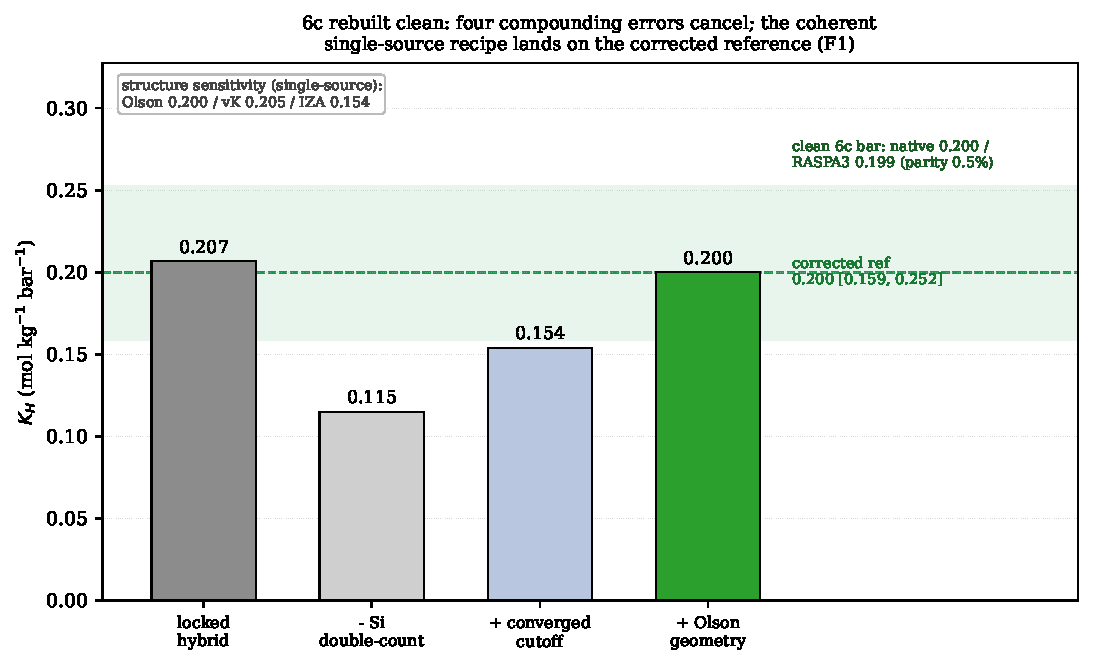
\includegraphics[width=0.78\textwidth]{figures/fp_6c_cancellation.pdf}
\caption{Finding F1 visualized: branch 6c rebuilt clean. The originally-locked hybrid recipe (\(0.207\))
agrees with the reference only as a fortuitous cancellation of four compounding errors; removing the silicon double-count,
converging the cutoff, and adopting Talu's calibration (Olson) geometry lands the coherent single-source
recipe on the corrected reference \(K_H = 0.200\), cross-engine (native \(0.200\), RASPA3 \(0.199\);
parity \(0.5\%\)). Values read from \texttt{cancellation\_6c.json}; the same chain is tabulated in
Table~\ref{tab:6c-cancellation}.}
\label{fig:6c-cancellation}
\end{figure}

\FloatBarrier

The same control provides, to our knowledge, the first published independent cross-engine validation of
the Widom test-particle estimator shipped in kUPS --- specifically the \texttt{kups.mcmc.widom} module,
as distinct from standalone Widom packages and from machine-learned-potential adsorption benchmarks such
as ODAC25~\cite{ODAC25}. The estimator is present in the engine source; a search of that source
found internal unit tests only, and the open issue tracker, inspected on 2026-06-12, carried one
unrelated feature request. On
two locked controls --- MFI + Ar without electrostatics, and Si-CHA + CO\(_2\) with framework charges and
Ewald summation --- kUPS reproduces the isosteric heat to \(0.22\) and \(0.01\) kJ/mol respectively; its
energies and its \(W=\exp(-\beta U)\) reduction are correct. The dominant \(K_H\) discrepancies trace to
named conventions: a \(+16\%\) gap on the Ar control root-causes to an LJ truncation convention (kUPS
truncates the potential at the cutoff where the reference shifts it; matching the convention reproduces
kUPS to \(+2.4\%\)), and the electrostatic control carries an additional tail-implementation difference.
One residual of order \(8\%\) remains, characterized as a normalization-flavoured, \(Q_{st}\)-invariant
scale and flagged open rather than hand-waved. Neither engine is wrong; the truncation convention is a
recipe element worth \(16\%\) on \(K_H\). The exponential sensitivity of \(K_H\) to a constant energy
offset, and the resulting need to lock the tail/truncation convention, are established
\cite{Jablonka2019,Dubbeldam2016}; what is new here is the cross-engine \emph{quantification} of the
effect, and the governed comparison is what makes it visible (Figure~\ref{fig:v06-parity}). The recipe these three engines share for this parity is the as-locked
hybrid reframed above as a silicon double-count; this does not weaken the validation, which tests whether
independent estimators agree on a \emph{common} recipe, not whether that recipe reproduces experiment. On the
convention-matched shifted recipe the native estimator and RASPA3 agree to \(1.1\%\) on \(K_H\); \(Q_{st}\) is
far less sensitive to the LJ shift convention, so kUPS stays within \(0.22\) kJ/mol of RASPA3 on the same
control even though its \(K_H\) carries the \(+16\%\) shifted-versus-truncated convention offset quantified above. The experimental-reproduction
correction --- silicon, structure, convention, reference --- lives entirely in the rebuilt control above;
the two findings are consistent.

\begin{figure}[tbp]
\centering
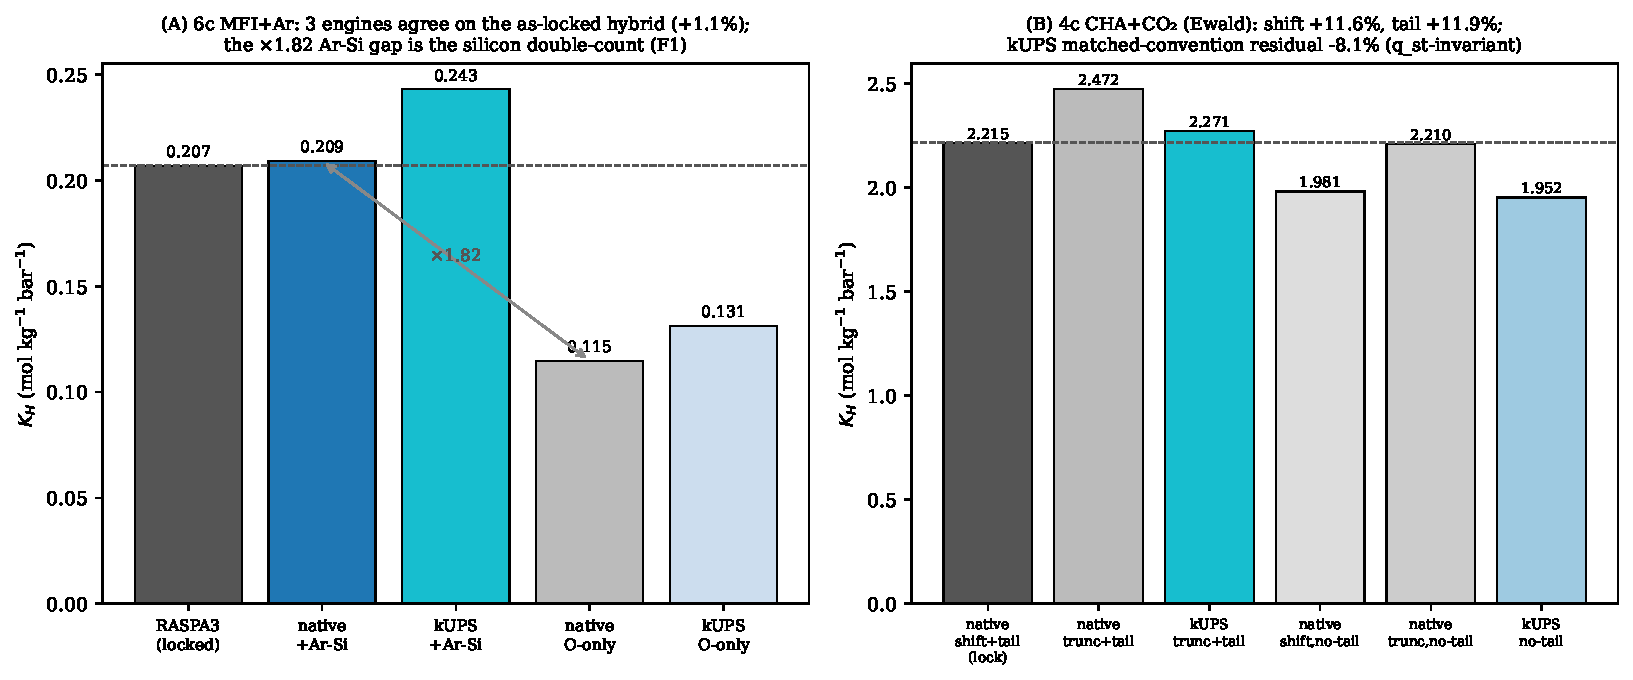
\includegraphics[width=\textwidth]{figures/fp_cross_engine_parity.pdf}
\caption{Cross-engine Widom parity. Left: on MFI + Ar, two independent estimators agree on the as-locked
hybrid recipe --- native + Ar--Si reproduces the locked RASPA3 reference --- and the factor-\(1.8\) gap to
the oxygen-only recipe is the silicon double-count of Finding~F1 quantified, not a legitimate missing
term. Right: the Si-CHA + CO\(_2\) (Ewald) convention matrix, isolating the LJ truncation shift and the
tail-implementation difference that account for the kUPS--reference offset.}
\label{fig:v06-parity}
\end{figure}

\FloatBarrier

\subsection{Machine-learned potentials as governed recipes}\label{sec:v06-mlip}

Treating an MLIP as one more energy-model recipe, we score Widom insertions of Ar into all-silica CHA
under four configurations, with a classical Lennard-Jones baseline scoring the same insertion geometries
so that every difference is the potential, not the sampling. The governance is a rule-based schema,
written before the results were seen and applied with one documented post-hoc correction (a spurious
weight clip, removed),
with two refusal classes: out-of-distribution over-binding (flagged insertions carry at least half the
Boltzmann weight) and absent-well under-binding (no physisorption minimum where one is established).
The second class is named for the observation rather than a mechanism: a flat positive plateau is
consistent with a missing dispersion term but equally with an unquantified out-of-distribution energy
offset, and the evidence here does not separate the two. The result
discriminates two distinct failure modes and, for one of them, certifies a governed screen-pass (Figure~\ref{fig:v06-triptych}). The 2023
MACE-MP-small potential hallucinates attractive energies \emph{inside} atomic overlaps --- its global
minimum, \(-19.3\) kJ/mol, lies at a hard overlap, and the flagged insertions carry \(99.5\%\) of the
weight; it is refused. The MACE-MPA-0 potential as shipped in CuspAI's \texttt{kUPS-mace-jax} export is
the opposite: repulsive everywhere (minimum \(+8.5\) kJ/mol), finding no physisorption well at all ---
consistent with the bare PBE signature of a missing dispersion term, although the plateau is flat with
distance and an out-of-distribution offset is not excluded; it too is refused. Pairing the \emph{same} weights with
the standard D3(BJ) dispersion correction recovers a physical well (minimum \(-5.0\) kJ/mol, shallower than the
\(-22\) kJ/mol classical baseline) at a non-overlap distance: it passes the out-of-distribution screen, accuracy
unassessed. Dispersion-correction on or off is therefore
a load-bearing recipe element, and an ungoverned pipeline silently differs on it. The kUPS in-engine JAX
export was verified energy-identical to the upstream reference implementation to a maximum relative
difference of \(2.1\times10^{-7}\), so the governance conclusions carry to the runtime path.

\paragraph{Audit correction to the overlap threshold.} The hard-overlap flag was applied at
\(0.80\,\sigma_{\min} = 2.762\)~\AA{}, built from \(\tfrac{1}{2}(3.500 + 3.405)\)~\AA{}. Those lengths
are not in the same convention: \(3.500\)~\AA{} is UFF's \(x_i\) for oxygen, which is \(r_{\min}\) and
not \(\sigma\) (\(\sigma = x_i/2^{1/6} = 3.118\)~\AA{}), while \(3.405\)~\AA{} is a Lennard-Jones
\(\sigma\) for argon. Re-derived self-consistently the threshold is \(2.626\)~\AA{}. Re-scoring the
committed per-insertion evidence changes no refuse or screen-pass verdict, but the UMA materials-head
flagged weight falls from \(0.998\) to \(0.000\), because its deepest insertion lies at \(2.646\)~\AA{}
--- inside the as-run overlap region and outside the corrected one. That refusal is therefore carried by
the energetic-anomaly gate, not the overlap gate, and the accurate description is that the potential is
erratic irrespective of overlap. A continuous \(U(r)\) scan along the line from the nearest framework
oxygen through that insertion confirms this: the anomaly is a smooth spurious basin reaching
\(-309.8\) kJ/mol at a host--guest separation of \(2.73\)~\AA{}, where the classical comparator on the
same trajectory is repulsive, and it reproduces on repeat to \(0.0005\) kJ/mol and shifts by a constant
\(0.195\) kJ/mol under a second reference configuration. The companion report carries the scan and the
full re-scoring. This is a \(\sigma \leftrightarrow r_{\min}\) slip of exactly the kind this paper is
about, caught by audit rather than by inspection.

\begin{figure}[tbp]
\centering
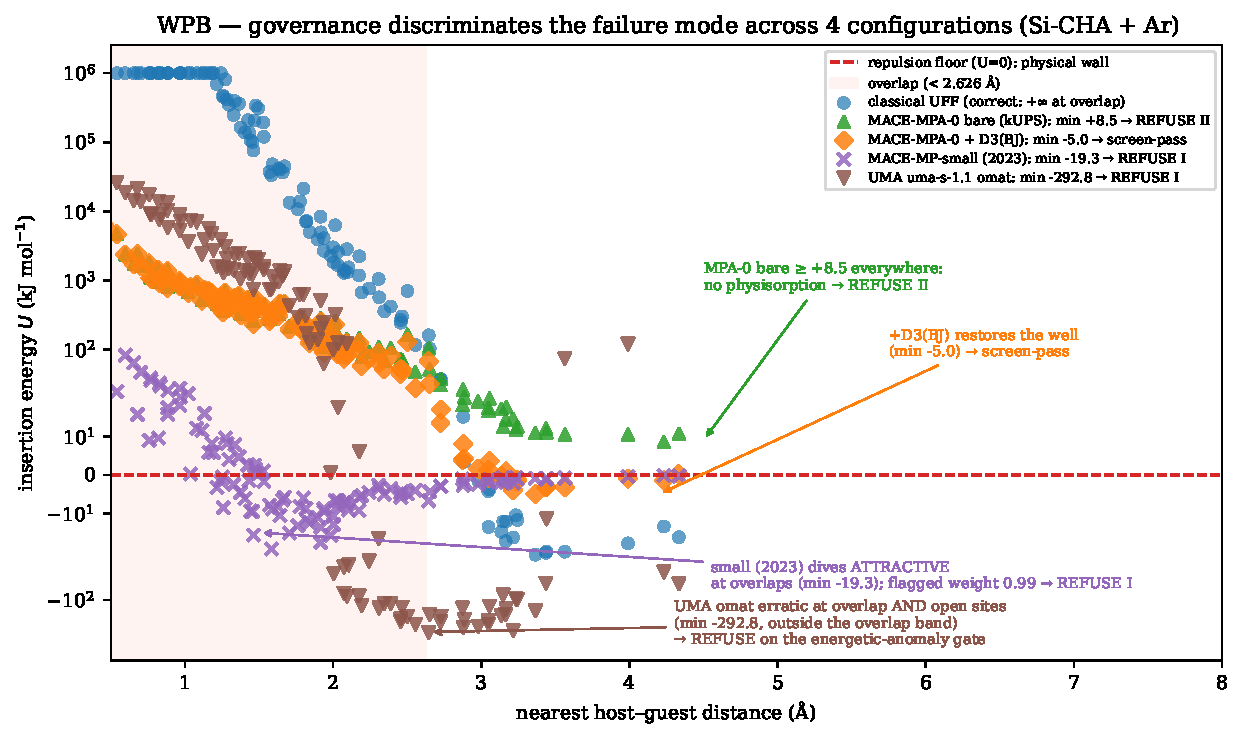
\includegraphics[width=\textwidth]{figures/f1_wpb_triptych.pdf}
\caption{Out-of-distribution governance discriminates the failure mode across four configurations
(Si-CHA + Ar). MACE-MP-small over-binds inside overlaps (refused); MACE-MPA-0 bare is repulsive
everywhere, finding no physisorption well (refused); the same weights with D3(BJ) recover a physical well
(screen-pass); the UMA materials head is erratic both inside and outside the overlap region and is
refused on the energetic-anomaly gate. The shaded band is the corrected \(2.626\)~\AA{} hard-overlap
threshold. Every label renders from a committed JSON.}
\label{fig:v06-triptych}
\end{figure}

\FloatBarrier

A multi-task foundation model sharpens the point that a verdict is only as good as the harness's right to
issue it. The UMA potential carries several level-of-theory heads; its choice is itself a recipe element.
Its materials head, used on Ar in silica, is erratic at close contact and is refused. Its direct-air-capture
head, used on Ar --- a noble gas outside its training distribution --- assigns energies that differ by
\(2.7\) kJ/mol between symmetry-equivalent open sites; the harness fails its own internal consistency
check and returns \emph{withheld}: no verdict, rather than a confident wrong one. The \emph{same}
direct-air-capture head, used on CO\(_2\) in the same framework --- CO\(_2\) is adsorbate-in-domain for this
head, though the all-silica CHA host lies outside the MOF host class used in its training --- is
self-consistent and finds a physical well (minimum \(-15.7\) kJ/mol, screen isosteric heat \(17.7\) kJ/mol
against a reference anchor of \(21.0\)): it passes the screen (Figure~\ref{fig:v06-uma}). The model passes
where its own documentation says it should, and is refused or withheld elsewhere. A screen-pass is not a
certificate of accuracy --- the runs are screens at \(N=60\)--\(120\) insertions, not converged
thermodynamics --- but it is the difference between a number that may be trusted and one that must not.

\begin{figure}[tbp]
\centering
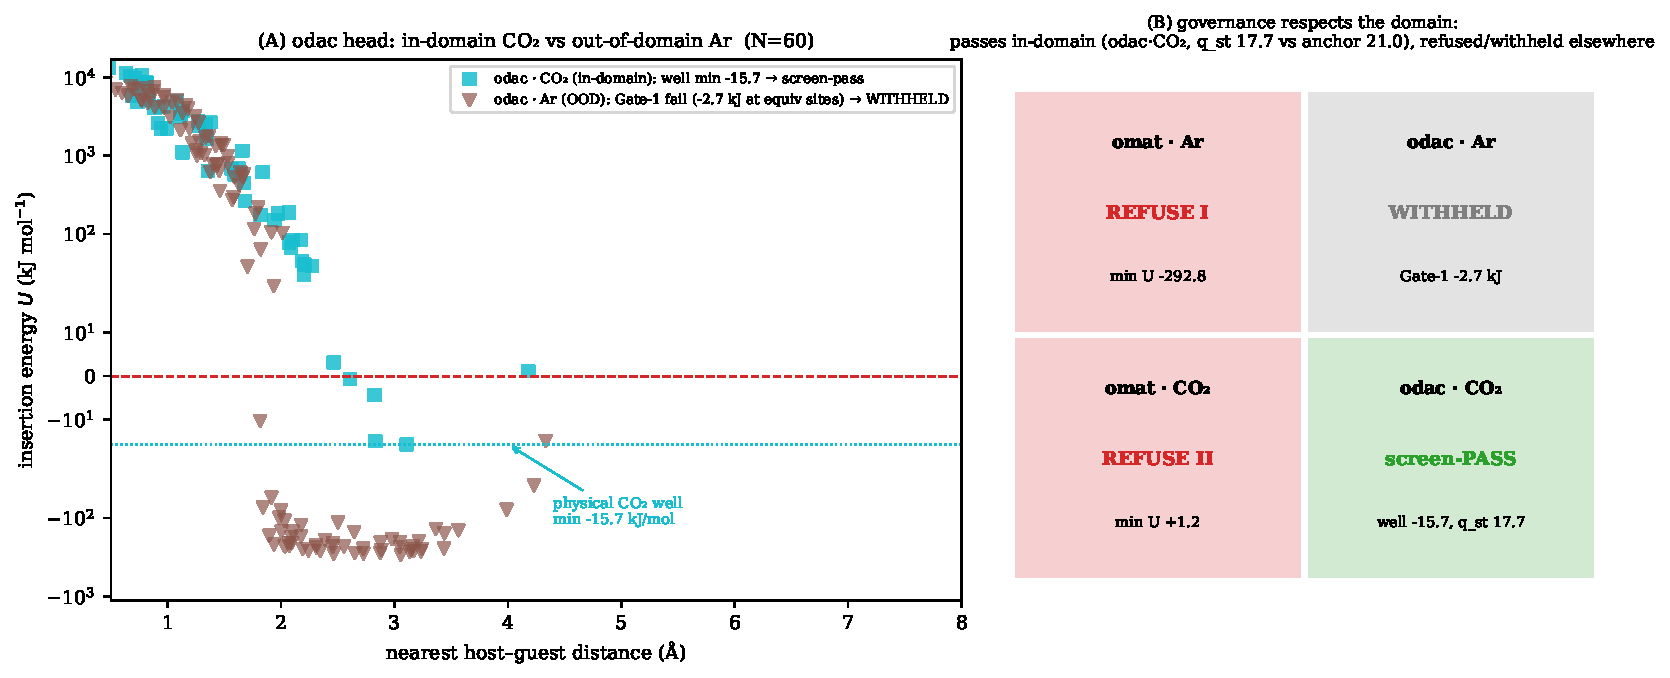
\includegraphics[width=\textwidth]{figures/f2_uma_domain.pdf}
\caption{Governance respects the model's domain. Left: the UMA direct-air-capture head screen-passes on
CO\(_2\) (adsorbate-in-domain; a physical well) and is withheld out-of-domain on Ar (internally inconsistent).
Right: the full task-by-system verdict matrix; the model passes where its adsorbate domain holds and is
refused or withheld elsewhere.}
\label{fig:v06-uma}
\end{figure}

\FloatBarrier

None of this changes the v0.4 verdict. It extends the same discipline to a second engine and to
machine-learned energy models, and it adds two recipe elements to the list that must be locked before a
Widom number is trustworthy: the engine's truncation convention, and the potential's domain of validity.
The point is unchanged. The trustworthy quantity is not the number; it is the number together with the
complete, locked recipe that produced it.
